\documentclass[fin1, tisk]{fmfdelo}
%\documentclass[mat1, tisk]{fmfdelo}
% Če pobrišete možnost tisk, bodo povezave obarvane,
% na začetku pa ne bo praznih strani po naslovu, …

%%%%%%%%%%%%%%%%%%%%%%%%%%%%%%%%%%%%%%%%%%%%%%%%%%%%%%%%%%%%%%%%%%%%%%%%%%%%%%%
% METAPODATKI
%%%%%%%%%%%%%%%%%%%%%%%%%%%%%%%%%%%%%%%%%%%%%%%%%%%%%%%%%%%%%%%%%%%%%%%%%%%%%%%

% - vaše ime
\avtor{Peter Milivojević}

% - naslov dela v slovenščini
\naslov{Igre ustvarjanja omrežji}

% - naslov dela v angleščini
\title{Network creation games}

% - ime mentorja/mentorice s polnim nazivom:
%   - doc.~dr.~Ime Priimek
%   - izr.~prof.~dr.~Ime Priimek
%   - prof.~dr.~Ime Priimek
%   za druge variante uporabite ustrezne ukaze
\mentor{prof.~dr.~Sergio Cabello Justo}
% \somentor{...}
% \mentorica{...}
% \somentorica{...}
% \mentorja{...}{...}
% \somentorja{...}{...}
% \mentorici{...}{...}
% \somentorici{...}{...}

% - leto diplome
\letnica{2024} 

% - povzetek v slovenščini
%   V povzetku na kratko opišite vsebinske rezultate dela. Sem ne sodi razlaga
%   organizacije dela, torej v katerem razdelku je kaj, pač pa le opis vsebine.
\povzetek{...}

% - povzetek v angleščini
\abstract{...}

% - klasifikacijske oznake, ločene z vejicami
%   Oznake, ki opisujejo področje dela, so dostopne na strani https://www.ams.org/msc/
\klasifikacija{..., ...}

% - ključne besede, ki nastopajo v delu, ločene s \sep
\kljucnebesede{...\sep ...}

% - angleški prevod ključnih besed
\keywords{...\sep ...} % angleški prevod ključnih besed

% - angleško-slovenski slovar strokovnih izrazov
\slovar{
% \geslo{angleški izraz}{slovenski izraz}
% ...
}

% - ime datoteke z viri (vključno s končnico .bib), če uporabljate BibTeX
% \literatura{....bib}

%%%%%%%%%%%%%%%%%%%%%%%%%%%%%%%%%%%%%%%%%%%%%%%%%%%%%%%%%%%%%%%%%%%%%%%%%%%%%%%
% DODATNE DEFINICIJE
%%%%%%%%%%%%%%%%%%%%%%%%%%%%%%%%%%%%%%%%%%%%%%%%%%%%%%%%%%%%%%%%%%%%%%%%%%%%%%%

% naložite dodatne pakete, ki jih potrebujete
% \usepackage{...}
\usepackage{graphicx}

% deklarirajte vse matematične operatorje, da jih bo LaTeX pravilno stavil
% \DeclareMathOperator{\...}{...}

% vstavite svoje definicije ...
% \newcommand{\...}{...}

%%%%%%%%%%%%%%%%%%%%%%%%%%%%%%%%%%%%%%%%%%%%%%%%%%%%%%%%%%%%%%%%%%%%%%%%%%%%%%%
% ZAČETEK VSEBINE
%%%%%%%%%%%%%%%%%%%%%%%%%%%%%%%%%%%%%%%%%%%%%%%%%%%%%%%%%%%%%%%%%%%%%%%%%%%%%%%

\begin{document}

\section{Uvod}

Namen diplomske naloge se je spoznati z igrami ustvarjanja omrežja s poudarkom na dve osnovni verziji tega problema.
V igri ustvarjanja omrežja imamo igralce, predstavljene kot vozlišča v grafu, ki želijo s 'sebično' izbiro svoje
strategije izboljšati svoj položaj. Običajno ima vsak igralec dva sebična cilja. Prvi cilj je minimizirat stroške
ustvarjanja povezav (omrežja) in drugi je minimizirat razdaljo, do ostalih vozlišč (strošek uporabe omrežja).


V osnovnih igrah omrežji predpostavimo, da se ne da primerjati cene ustvarjanja in vzdrževanja povezav. Zato se
omejimo na že v naprej podane grafe (omrežja), kjer lahko vozlišča (igralci) le zamenjajo svoje povezave ali v
posebnem primeru odstranijo povezavo, tako da zamenjajo pvezavo za že obstoječo povezavo, s čimer se ena povezava
izbriše, saj se bomo ukvarjali le zgrafi brez zank in dvojnih povezav. Ne morejo pa ustvarit novih povezav.

\section{Teoretična podlaga}
Da bomo lahko razumeli obnašanje igralcev in lastnosti nastalih omrežji bomo prvo obnovili/postavili teoretične temelje. 
Ukvarjali se bomo izključno z povezanimi enostavnimi grafi.

Za lažje razumevanje nadaljnih izrekov, lem, trditev, posledic in rezultatov bomo ponovili nekaj definicij o grafih.

\begin{definicija}
$Graf$ je urejen par G = (V, E), kjer je V neprazna množica točk grafa G in E množica povezav grafa G, pričemer je vsaka povezava par točk.
\end{definicija}

\begin{definicija}
$Graf$ G je povezan, če za vsak par voclišč $u, v \in V(G)$ obstaja pot od $u$ do $v$.
\end{definicija}

\begin{definicija}
Naj bo $G$ povezan graf in $v \in V(G)$. Stopnja točke $v$ je enaka vsoti števila povezav, ki imajo to točko za krajišče (in dvojnega števila zank v tej točki).
Označimo jo z $deg(v)$.
\end{definicija}

\begin{definicija}
Naj bo $G$ povezan graf in $u, v \in V(G)$. Razdalja $d(u, v)$ je dolžina najkrajše poti med vozliščema $u$ in $v$ (t.j. razdalja med $u$ in $v$) v grafu $G$.
\end{definicija}

\begin{definicija}
Naj bo $G$ povezan graf. Premer grafa $G$ je definiran kot $\text{diam}(G) = \max_{u, v \in V(G)} d(u, v)$, kjer je $d(u, v)$ razdalja med vozliščema $u$ in $v$ v grafu $G$.
\end{definicija}

\begin{definicija}
Naj bo $G$ povezan graf. Lokalni premer točke $v$ grafa $G$ je definiran kot $\text{diam}(G) = \max_{u \in V(G)} d(u, v)$, kjer je $d(u, v)$ razdalja med vozliščema $u$ in $v$ v grafu $G$.
\end{definicija}

\begin{definicija}
Povezan graf $G$ ima prerezno vozlišče $v$, če graf $G - v$ ni povezan.
\end{definicija}

%\begin{definicija}
%Povezanost po povezavah $\lambda(G)$ povezanega grafa $G$ je najmanjše število povezav,
%z odstranitvijo katerih postane graf $G$ nepovezan. Če je $\lambda(G) \geq k$,
%je graf $G$ po povezavah $k$-povezan.
%\end{definicija}

Weinerjev indeks nam bo pomagal z kasnejšimi dokazi.

\begin{definicija}
Naj bo $G$ povezan graf z n vozlišči. Weinerjev indeks $W = W(G)$ je definiran
kot vsota vseh razdalj med vozlišči.
$$W(G) = \sum_{i=1}^{n} \sum_{j=1}^{i} d_{ij} = \frac{1}{2} \sum_{i=1}^{n} \sum_{j=1}^{n} d_{ij}$$
kjer $d_{ij}$ označuje dolžino najkrajše poti med vozliščem $i$ in $j$.
\end{definicija}

\section{Igra}
Pomembno za razumevanje kasnejših delov diplomske naloge je tudi razumevanje kaj je igra v smislu teorije iger.


!!!!!!!!!


\begin{definicija}
    Strateška igra s funkcijo preferenc je trojica $(N, (A_i)_{i\in N} , (u_i)_{i\in N})$ pri čemer:
\begin{itemize}
    \item $N$ je množica igralcev, v našem primeru je to število točk v grafu
    \item Za vsakega igralca $i \in N$ je $A_i$ neprazna množica njegovih akcij, med katerimi v danem trenutku izbera igralec $i$
    \item Za vsakega igralca $i \in N$ je $u_i$ funkcija preferenc na $A_i$. Torej $u_i : A_i \to \mathbb{R}$ v splošnem in $u_i : A_i \to \mathbb{N}$ v našem primeru.
\end{itemize}
\end{definicija}
Za funkcijo preferenc lahko zapišemo sledeče relacije.

$\forall a,b \in A_i:$
\begin{itemize}
    \item $(u(a) \geq u(b) \Rightarrow a)$ je vsaj tako dobro kot $b$
    \item $(u(a) > u(b) \Rightarrow a)$ je boljše kot $b$
    \item $(u(a) = u(b) \Rightarrow b)$ indiferenten med $a$ in $b$
\end{itemize}


\section{Ravnovesje}
V tem delu bomo definirali pravila igre in pogoje za nastanek ravnovesji.

\begin{definicija}
Graf je v \textit{ravnotežju glede na vsoto razdalj}, če za vsako povezavo $vw$ in
za vsako vozlišče $w'$ zamenjava povezave $vw$ z povezavo $vw'$ ne zmanjša
celotne vsote razdalj od vozlišča $v$ do vseh ostalih vozlišč.
\end{definicija}

\begin{definicija}
Graf je v \textit{ravnotežju glede na maksimalno razdaljo}, če za vsako povezavo $vw$
in za vsako vozlišče $w'$ zamenjava povezave $vw$ z povezavo $vw'$ ne zmanjša
lokalnega premera vozlišča $v$. Nadalje odstranitev povezave $vw$ poveča
lokalni premer vozlišča $v$.
\end{definicija}


\begin{definicija}
Naj bo $G$ povezan graf. Graf $G$ je \textit{kritičen za odstranitev povezave},
če odstranitev katere koli povezave $uv \in E(G)$ poveča lokalni premer vozlišča $v$ in vozlišča $u$.
\end{definicija}

\begin{definicija}
Naj bo $G$ povezan graf. Graf $G$ je \textit{stabilen za dodajanje povezave},
če dodajanje katere koli povezave $uv \in E(G)$ ne zmanjša lokalnega premera vozlišča $v$ in vozlišča $u$.
\end{definicija}

\section{Cena anarhije in cena stabilnosti}
V delu se bomo ukvarjalise tudi z ceno anarhije (PoA) in ceno stabilnosti (PoS).
Ceni anarhije in stabilnosti merita, kako se učinkovitost sistema poslabša zaradi sebičnega vedenja njegovih agentov.
Cena anarhije je razmerje med vrednostjo/ceno, iz socialnega vidika (skupnega vidika vseh igralcev), najslabšega ravnovesja in socialno ceno optimalnega izida
Cena stabilnosti igre pa je razmerje med najboljšo socialno ceno ravnovesja in socialno ceno optimalnega izida.\\
Socialno ceno grafa bomo definirali kot vsoto cen vseh vozlišč. Za igro vsote bomo tako socialno ceno definirali kot $SC(G) = 2W(G)$,
za igro lokalnega premera pa kot $SC(G) = \sum_{i=1}^{n}\epsilon_G(i)$.
Tako lahko definiramo sledeče:
\begin{definicija}
$PoA = \frac{\text{Socialna cena najslabšega ravnovesja}}{\text{Socialna cena optimalne postavitve}} = \frac{\max_{G\in R} SC(G)}{\min_{G\in A} SC(G)}$
\end{definicija}
\begin{definicija}
$PoS = \frac{\text{Socialna cena najboljšega ravnovesja}}{\text{Socialna cena optimalne postavitve}} = \frac{\min_{G\in R} SC(G)}{\min_{G\in A} SC(G)}$
\end{definicija}
Kjer $A$ predstavlja množico vseh možnih povezanih grafov z $|V(G)| = n$ vozlišči in manj ali enako kot $|E(G)| = m$ povezavami.
Množica $R \subseteq A$ pa predstavlja množico vseh ravnovesnih grafov, ki lahko nastanejo iz začetnih grafov z $n$ vozlišči in $m$ povezavami.





\section{Teoretični del diplomske naloge}

Nekoliko zahtevnejši in bolj raznoliki grafi od polnih grafov so drevesa.

\begin{izrek}
Če je ravnovesni graf za skupno vsoto razdalj v preprosti igri ustvarjanja
omrežja drevo, potem ima premer največ $2$ in je kot tak zvezda.
\end{izrek}

\begin{dokaz}
Dokaza se bomo lotili z protislovjem. Predpostavimo, da je ravnovesni graf
drevo s premerom 3 ali več. Ker ima premer vsaj 3 obstajata vozlišči
$u$ in $v$ oddaljeni eno od druge za točno 3 preko najkrajše in edine poti,
ki gre skozi dve točki, ki jih označimo z $a$ in $b$. Tako imamo pot
$v \to a \to b \to u$. Z $s_v,\ s_a,\ s_b,\ s_u$ označimo število morebitnih
točk poddreves upetih na $v, a, b, u$. Obravnavamo 2 možni zamenjavi: 
\end{dokaz}

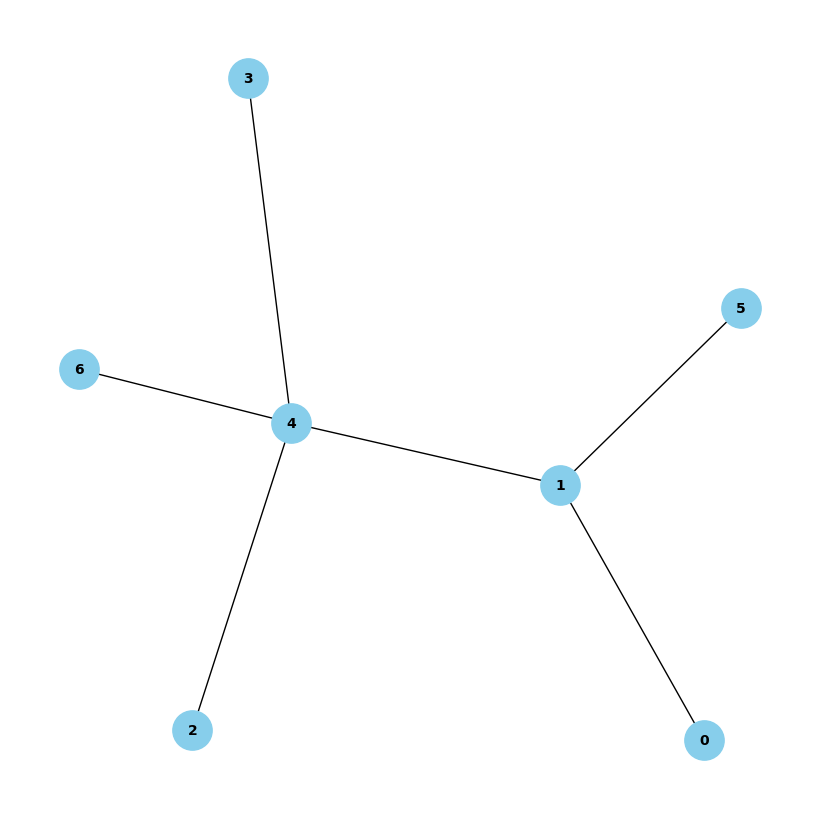
\includegraphics[width=0.3\textwidth]{drevo_1.png}
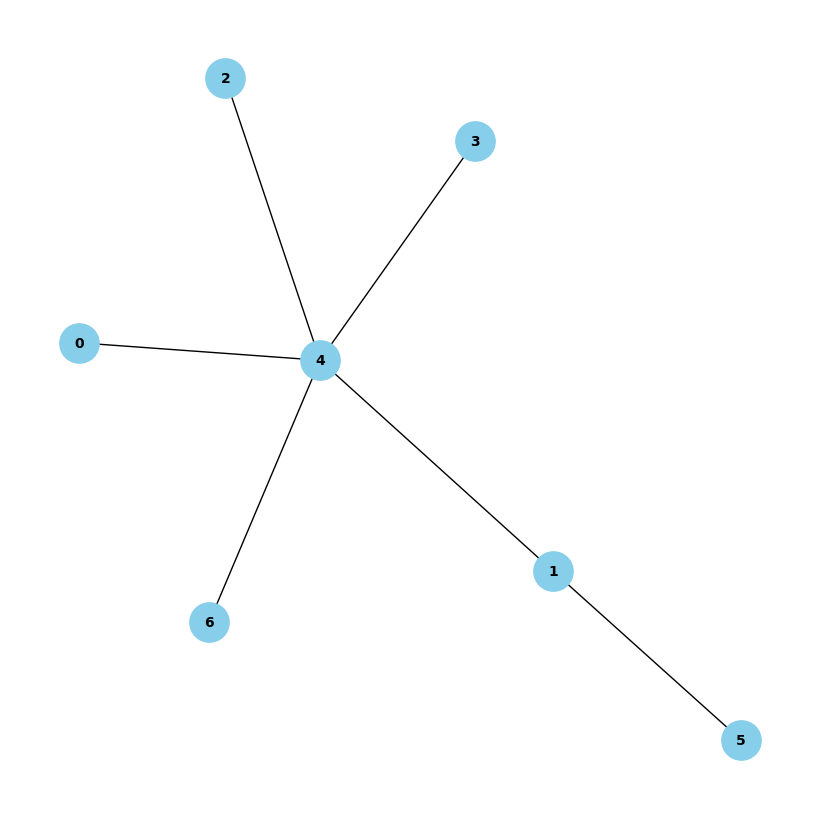
\includegraphics[width=0.3\textwidth]{drevo_2.png}
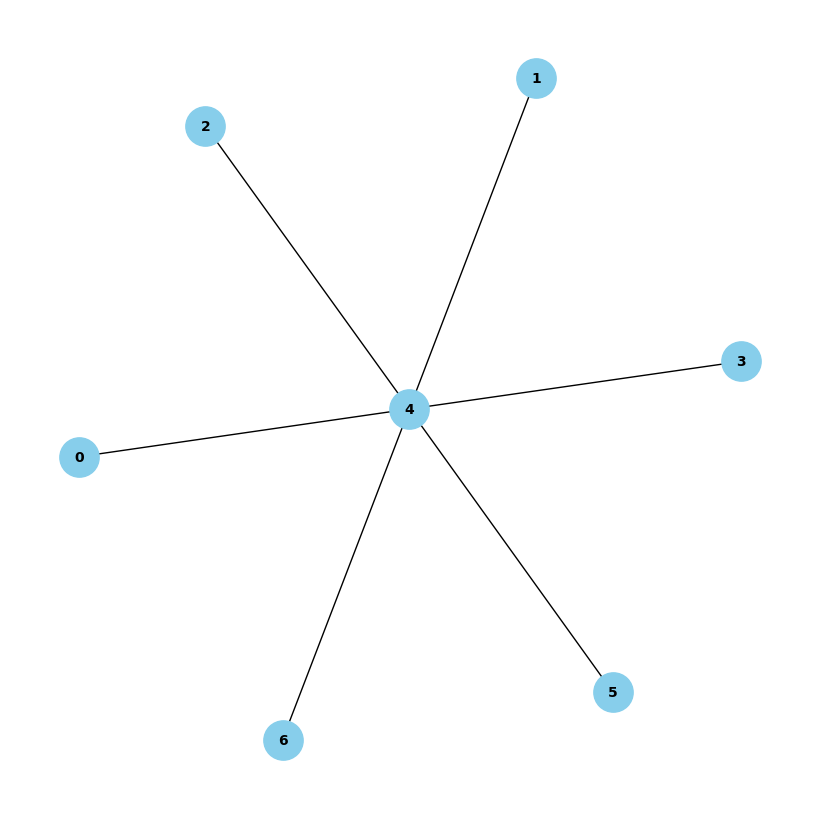
\includegraphics[width=0.3\textwidth]{drevo_3.png}


\begin{lema}
V vsakem ravnovesnem grafu igre maksimalne razdalje se lokalni premer za
katera koli $2$ poljubna vozlišča razlikuje največ za $1$.
\end{lema}

\begin{dokaz}
Predpostavimo, da je graf v \textit{ravnotežju glede na maksimalno razdaljo} in ima vozlišče $v$ z lokalnim premer $d$ in vozlišče
$w$ z lokalnim premerom vsaj $d+2$. Naj bo $T$ drevo, ki ga dobimo z iskanjem v širino
iz vozlišča $v$. Vozlišče $w$ z zamenjavo svoje povezave s staršem v $T$ z povezavo do
$v$ (korena $T$) zmanjša svoj lokalni premer. Opazimo, da ta zamenjava lahko le zmanjša ali ohrani globine vozlišč v $T$,
zato lokalni premer vozlišča $v$ ostane največ $d$. Tako se lokalni premer
vozlišča $w$ zmanjša na vsaj $d+1$, saj se $w$ lahko premakne po novo nastali povezavi $wv$ do
$v$ in nato sledi poti $v$ do vseh ostalih vozlišča. Ta zamenjava
je v nasprotju s predpostavko, da je graf v \textit{ravnotežju glede na maksimalno razdaljo} saj lahko vozlišče $u$
izboljša svoj položaj(zmanjša svoj lokalni premer) z omenjeno zamenjavo povezav.
\end{dokaz}

\begin{lema}
Če ima ravnovesni graf za maksimalno razdaljo prerezno vozlišče $v$, potem ima lahko
samo ena izmed povezanih komponent $G - v$ vozlišče z razdaljo več kot $1$ od $v$.
\end{lema}

\begin{dokaz}
Ponovno bomo dokazali lemo z protislovjem. Naj bo $d$ lokalni premer prereznega vozlišča $v$
in naj bo vozlišče $u$ na razdalji $d$ od $v$. Z $U$ označimo povezano komponento $G - v$ ki vsebuje $u$.
Predpostavimo, da $G - U$ vsebuje vozlišče $z$, ki je za več kot $1$ oddaljeno od vozlišča $v$. Ker je vozlišče $v$
prerezno in $z$ in $u$ nista vozlišči iste povezane komponente $G - v$, mora vsaka pot med njima prečkati $v$.
Tako je najkrajša pot od $z$ do $u$ dolga $d + 2$. Lokalni premer $z$ in $u$ je zato vsaj $d + 2$
kar se za več kot $1$ razlikuje od lokalnega premera vozlišča $v$ in je tako v nasprotju z predhodno lemo
in zato graf, ki ima več kot eno povezano komponento $G - v$ z vozliščem z razdaljo več kot $1$ od $v$,
ne more biti ravnovesni graf.
\end{dokaz}

\begin{izrek}
Če je ravnovesni graf za maksimalno razdaljo drevo, potem ima premer največ $3$.
\end{izrek}


\begin{dokaz}
Predpostavimo, da je ravnovesni graf za maksimalno razdaljo drevo in ima premer vsaj $4$.
Potem obstajata vozlišči $v$ in $u$, ki sta na razdalji točno $4$ in med njima obstaja pot dolžine $4$
$v \to a \to b \to c \to u$. Ker je graf drevo je vozlišče $b$ prerezno vozlišče z dvema
povezanima komponentama $G - b$, ki vsebujeta vozlišči $v$ in $u$, ki sta na razdalji več kot $1$ od $b$
in tako v protislovju z predhodno lemo.
\end{dokaz}


\begin{lema}
Za vozlišče $v$ z lokalnim premerom $2$, zamenjava sosednje povezave ne izboljša
vsote razdalj od $v$ do vseh ostalih voclišč. Prav tako tudi svojega lokalnega premera ne more izboljšati.
\end{lema}


\begin{dokaz}
Naj ima graf $G$ $n$ vozlišč in naj ima poljubno vozlišče z lokalnim premerom $2$
stopnjo $deg(v) = k$. Tako ima vozlišče $v$, $k$ sosednjih vozlišč in $n - k - 1$
vozlišč na razdalji $2$, saj je lokalni premer v enak $2$. Vsota razdalj od $v$
do vseh ostalih vozlišč je zato $1*k + 2*(n - k - 1)$.
Vozlišče $v$ z menjavo poljubne povezave ne spremeni števila sosednjih vozlišč $k$.
Zamenjavo ene izmed povezav vozlišča $v$ lahko tretiramo kot odstranitev ene
obstoječe povezave, s katero se izgubi eno sosedno vozlišče, in dodajo nove povezave,
s katero se pridobi eno sosednje vozlišče. Tako ima vozlišče $v$ ne glede na
zamenjavo povezav, $k$ sosednjih vozlišč in $n - k - 1$ vozlišč na razdalji vsaj $2$,
saj se razdalja do ne sosednjiega vozlišča lahko le poveča ali ostane enaka $2$.
Zato je vsota razdalj od $v$ do vseh ostalih voclišč, po zamenjavah povezav $v$
enaka ali večja od $1*k + 2*(n - k - 1)$.
\end{dokaz}





\begin{posledica}
!!!!!!!!!! Vsak graf z premerom $2$ ali manj je v \textit{ravnotežju glede na vsoto razdalj}.
In hkrati socialni optimum.
\end{posledica}

\begin{posledica}
Cena stabilnosti je 1.
\end{posledica}


\begin{izrek}
Naj bo $G$ graf z $n$ vozlišči in $m$ povezavami, potem je $W(G) = n^2 - n - m$, če in samo če je premer grafa $2$ ali manj.
\end{izrek}

\begin{dokaz}
Predpostavimo, da je $G$ graf reda $n$ in velikosti $m$ ter da velja $\text{diam}(G) \leq 2$.
Definirajmo množici $A = \{u \in V | e(u) = 1\}$ in $B = \{u \in V | e(u) = 2\}$. Potem velja $|A| + |B| = n$.
Če je $u \in A$, potem je $d(u) = n - 1$ (vsota vseh razdalj od $u$ do ostalih vozlišč), in če je $u \in B$,
definiramo dve množici $B_1$ in $B_2$ kot $B_1 = \{v \in V | d(u, v) = 1\}$ in $B_2 = \{v \in V | d(u, v) = 2\}$.

Nato velja:
\begin{align*}
d(u) &= |B_1| + 2|B_2| \\
&= |B_1| + |B_2| + |B_2| \\
&= n - 1 + (n - 1 - |B_1|) \qquad \text{ker} \ |B_1| + |B_2| = n - 1 \\
&= 2n - 2 - |B_1| \\
&= 2n - 2 - \text{deg}(u)
\end{align*}

In zato sledi:
\begin{align*}
W(G) &= \frac{1}{2} \sum_{u \in V} d(u) \\
&= \frac{1}{2}( \sum_{u \in A} d(u) + \sum_{u \in B} d(u)) \\
&= \frac{1}{2}( (n - 1)|A| + \sum_{u \in B} 2n - 2 - \text{deg}(u)) \\
&= \frac{1}{2}( (n - 1)|A| + (2n - 2)|B| - \sum_{u \in B} \text{deg}(u)) \\
&= \frac{1}{2}( (n - 1)(|A| + |B|) + (n - 1)|B| - \sum_{u \in B} \text{deg}(u)) \\
&= \frac{1}{2}( (n - 1)n + (n - 1)(n - |A|) - \sum_{u \in B} \text{deg}(u)) \\
&= \frac{1}{2}( (n - 1)n + (n - 1)n - (n - 1)|A| - \sum_{u \in B} \text{deg}(u)) \\
&= \frac{1}{2}( 2(n - 1)n  - \sum_{u \in A} \text{deg}(u)) - \sum_{u \in B} \text{deg}(u)) \\
&= \frac{1}{2}( 2(n - 1)n  - \sum_{u \in V} \text{deg}(u)) \\
&= \frac{1}{2}( 2(n - 1)n  - 2m) \qquad \text{ker} \ \sum_{u \in V} \text{deg}(u) = 2m, u \in V \\
&= n^2 - n - m \\
\end{align*}

Kar dokaže, da je $W(G) = n^2 - n - m$ za grafe s premerom manjšim od $2$ ($\text{diam}(G) \leq 2$). V drugem delu
bomo dokazali, da ta enakost ne velja za grafe z premerom večjim od $2$. Za graf $G$ ki ima premer vsaj $3$ (($\text{diam}(G) \geq 3$))
bomo definirali množici $A = \{u \in V | e(u) = 2\}$ in $B = \{u \in V | e(u) \geq 3\}$. Za kateri velja $|A| + |B| = n$.
Če je $u \in A$, potem iz zgoraj dokazanega velja $d(u) = 2n - 2 - \text{deg}(u)$.
Za $u \in B$ pa bomo definirali sledeče 3 podmnožice:


\begin{align*}
B_1 &= \{v \in V | d(u,v) = 1\}, \\
B_2 &= \{v \in V | d(u,v) = 2\}, \\
B_3 &= \{v \in V | d(u,v) \geq 3\}. \\
\text{Očitno, } |B_1| + |B_2| + |B_3| &= n - 1. \\
d(u) &\geq |B_1| + 2|B_2| + 3|B_3| \\
&= |B_1| + |B_2| + |B_3| + |B_2| + 2|B_3| \\
&= n - 1+ (n - 1 - |B_1|)+ | B_3| \\
&= 2n-2-\text{deg}(u) + | B_3| \\
&= 2n-2-\text{deg}(u) + | B_3| \\
&\geq 2n-2-\text{deg}(u)+1 \qquad \text{ saj } \ |B_3| \geq 1 \\
&\geq 2n-1-\text{deg}(u). \\
\therefore W(G) &= \frac{1}{2} \sum_{u \in V} d(u) \\
&=\frac{1}{2}(\sum_{u \in A} d(u) + \sum_{u \in B} d(u)) \\
&\geq \frac{1}{2}((\sum_{u \in A} (2n-2-\text{deg}(u))+(\sum_{u \in B} (2n-1-\text{deg}(u))) \\
&=\frac{1}{2}((2n-2)(|A| + |B|) - \sum_{u \in A} \text{deg}(u))-(\sum_{u \in B} \text{deg}(u))+ |B|) \\
&=\frac{1}{2}((2n-2)n - (\sum_{u \in V} \text{deg}(u)) + |B|) \\
&=\frac{1}{2}(2(n-1)n - 2m + |B|) \\
&=n(n - 1) - m + \frac{1}{2}|B| \\
&\geq n(n - 1) - m + 1  \qquad \text{ saj } \ |B| \geq 2
\end{align*}

\end{dokaz}


\begin{posledica}
Za vsak graf $G$ z $n$ vozlišči, $m$ povezavami in premerom večjim od $2$ velja:
$$W(G) \geq n^2 - n - m + 1.$$
Enačaj velja kadar ima graf $G$ natanko $2$ vozlišča z lokalnim premerom $3$ in vsa ostala vozlišča z lokalnim premerom $2$.
\end{posledica}

\begin{dokaz}

\end{dokaz}


\begin{izrek}
Obstaja ravnovesni graf za skupno vsoto razdalj s premerom $3$.
\end{izrek}

\begin{dokaz}
Graf na spodnji sliki ima premer $3$ in je v \textit{ravnotežju glede na vsoto razdalj}.
Točke $1$, $3$, $5$ in $7$ imajo lokalni premer $2$ in tako po predhodni lemi ne
morejo same zmanjšati svoje vsote razdalj do vseh ostalih vozlišč. Točke $2$, $4$,
$6$ in $8$ so simetrične in celo povezavi teh točk so simetrične, zato je dovolj
pogledati vse možne zamenjave le za eno izmed povezav teh točk. Točka $2$ ima
vsoto razdalj do vseh ostalih točk enako $1 + 1 + 2 + 2 + 2 + 2 + 3 = 13$. Za
preverjanje ali lahko točka $2$ izboljša svoj položaj bomo poskusili z zamenjavo
povezave med točkama $2$ in $1$ z novimi povezavami med točko $2$ in ostalimi povezavami.
Če povezavo $21$ zamenjamo s povezavo $24$ ima vozlišče $2$ vsoto razdalj enako
$1 + 1 + 2 + 2 + 3 + 3 + 3 = 15$. Če povezavo $21$ zamenjamo s povezavo $25$ ima
vozlišče $2$ vsoto razdalj enako $1 + 1 + 2 + 2 + 2 + 2 + 3 = 13$. Če povezavo $21$
zamenjamo s povezavo $26$ ima vozlišče $2$ vsoto razdalj enako
$1 + 1 + 2 + 2 + 2 + 3 + 3 = 14$. Če povezavo $21$ zamenjamo s povezavo $27$ ima
vozlišče $2$ vsoto razdalj enako $1 + 1 + 2 + 2 + 2 + 3 + 3 = 14$. Če povezavo $21$
zamenjamo s povezavo $28$ ima vozlišče $2$ vsoto razdalj enako
$1 + 1 + 2 + 2 + 2 + 3 + 3 = 13$.
\end{dokaz}

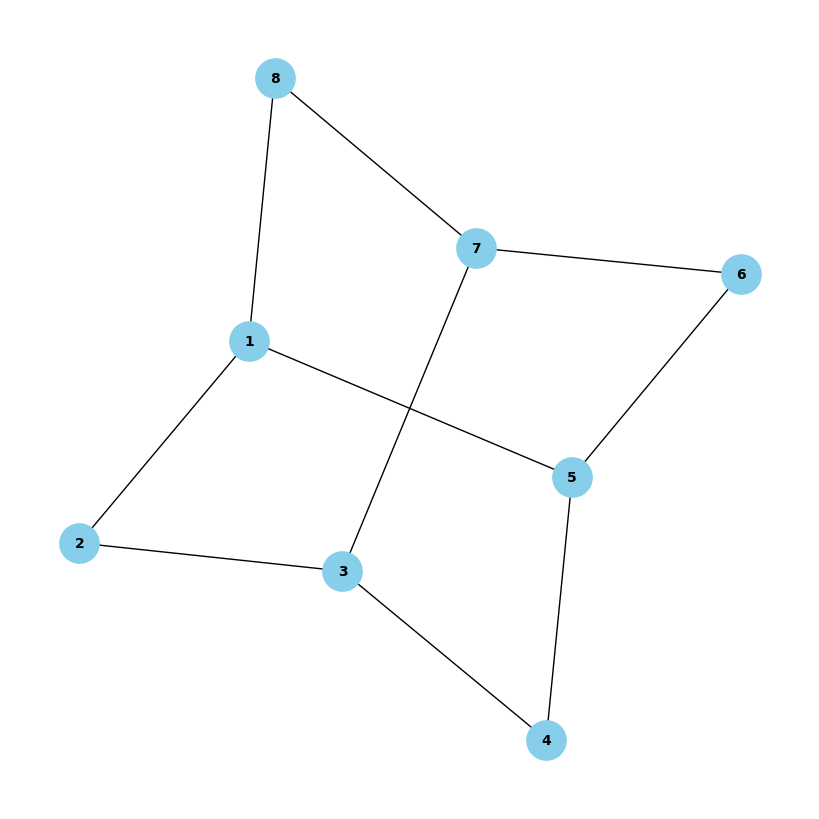
\includegraphics[width=0.9\textwidth]{vsota_premer_3.png}

\begin{izrek}
Vsak ravnovesni graf za skupno vsoto razdalj ima premer $2^{O(\sqrt{\lg n})}$.
\end{izrek}

\begin{lema}
Vsak ravnovesni graf za skupno vsoto razdalj ima premer največ $2 \lg n$ ali
za vsako vozlišče $v$ obstaja povezava $xy$ kjer je $d(u, x) \leq \lg n$ in
zamenjava povezave $xy$ zmanjša vsoto razdalj od $x$ za največ $2n(1 + \lg n)$.
\end{lema}

\begin{lema}
V vsakem ravnovesnem grafu za skupno vsoto razdalj dodajanje poljubne povezave
$uv$ zmanjša vsoto razdalj od $u$ za največ $5n \log n$.
\end{lema}

\begin{izrek}
Obstaja ravnovesni graf za maksimalno razdaljo z premerom $\Theta(\sqrt{n})$.
\end{izrek}
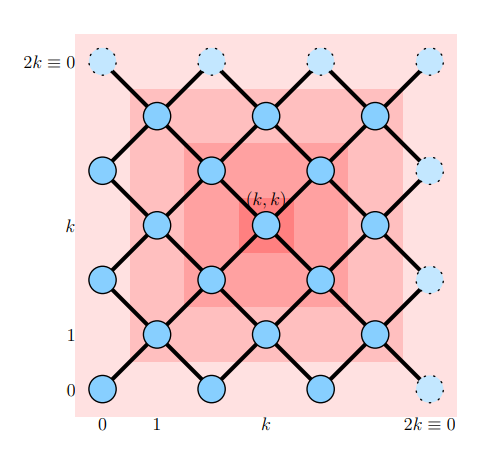
\includegraphics[width=0.9\textwidth]{Plagiat.png}


\begin{izrek}
Vsak ravnovesni graf za skupno vsoto razdaljo $G$ z $n \geq 24$ vozlišč in
premerom $d > 2 \lg n$ inducira podgraf z $\epsilon\text{-skoraj-enotno-razdaljo } G'$
z $n$ vozlišči in premerom $\Theta\left(\frac{\varepsilon d}{\lg n}\right)$ in
podgraf z $\epsilon\text{-enotno-razdaljo } G'$ z $n$ vozlišči in premerom
$\Theta\left(\frac{\varepsilon d}{\lg^2 n}\right)$.
\end{izrek}


\begin{izrek}
Vsak ravnovesni graf za osnovne igre ustvarjanja omrežji (mogoče samo za vsoto) ima največ eno po povezavah $2-$povezano komponento.
\end{izrek}

\begin{dokaz}
!!!!!!!!
\end{dokaz}


\section{Testiranje}

Lokalni premer verzija:

\begin{table}[]
\begin{tabular}{ll}
Št. ravnovesnih grafov & Št. vozlišč\\
1                      & 1          \\
1                      & 2          \\
2                      & 3          \\
3                      & 4          \\
4                      & 5          \\
7                      & 6          \\
12                     & 7          \\
24                     & 8          
\end{tabular}
\caption{Maks verzija}
\end{table}

Vsota razdalj verzija:

\begin{table}[]
\begin{tabular}{ll}
Št ravnovesji & Št. vozlišč\\
1             & 1          \\
1             & 2          \\
2             & 3          \\
5             & 4          \\
15            & 5          \\
60            & 6          \\
374           & 7          \\
4161          & 8         
\end{tabular}
\caption{Verzija vsote}
\end{table}




Socialni optimum max \\

\begin{table}[h]
    \centering
    \resizebox{\linewidth}{!}{%
        \begin{tabular}{|c|*{16}{c|}}
        \hline
        \multirow{\textbf{n$\backslash$e}} & \multicolumn{16}{c|}{\textbf{Število povezav}} \\ \cline{2-17}
        & \textbf{n - 1} & \textbf{n} & \textbf{n + 1} & \textbf{n + 2} & \textbf{n + 3} & \textbf{n + 4} & \textbf{n + 5} 
        & \textbf{n + 6} & \textbf{n + 7} & \textbf{n + 8} & \textbf{n + 9} & \textbf{n + 10} & \textbf{n + 11} & \textbf{n + 12} 
        & \textbf{n + 13} & \textbf{n + 14}\\
        \hline
            2 & (2, 'Je')  &            &            &            &            &            &            &            &            &            &            &            &            &            &           &           \\
            3 & (5, 'Je')  & (3, 'Je')  &            &            &            &            &            &            &            &            &            &            &            &            &           &           \\
            4 & (7, 'Je')  & (7, 'Ni')  & (6, 'Ni')  & (4, 'Je')  &            &            &            &            &            &            &            &            &            &            &           &           \\
            5 & (9, 'Je')  & (9, 'Ni')  & (9, 'Ni')  & (8, 'Ni')  & (8, 'Ni')  & (7, 'Ni')  & (5, 'Je')  &            &            &            &            &            &            &            &           &           \\
            6 & (11, 'Je') & (11, 'Ni') & (11, 'Ni') & (11, 'Ni') & (10, 'Ni') & (10, 'Ni') & (10, 'Ni') & (9, 'Ni')  & (9, 'Ni')  & (8, 'Ni')  & (6, 'Je')  &            &            &            &           &           \\
            7 & (13, 'Je') & (13, 'Ni') & (13, 'Ni') & (13, 'Ni') & (13, 'Ni') & (12, 'Ni') & (12, 'Ni') & (12, 'Ni') & (12, 'Ni') & (11, 'Ni') & (11, 'Ni') & (11, 'Ni') & (10, 'Ni') & (10, 'Ni') & (9, 'Ni') & (7, 'Je') \\
        \hline
        \end{tabular}
    }
    \caption{Your table caption goes here.}
    \label{tab:tabela2}
\end{table}\\


Premer grafa je največ 2. Vozlišča s premerom 2 bi si želela odstraniti nekatere povezave.
Cena stabilnosti je lahko večja od 1 ampak manjša od 2. Ko gre n proti neskončno konvergira proti 2 ali 1.
!!!!!! Optimalni grafi se stabilizirajo kot zvezde za max.


Socialni optimum sum, (opti, premer)\\
\begin{table}[h]
    \centering
    \resizebox{\linewidth}{!}{%
        \begin{tabular}{|c|*{16}{c|}}
        \hline
        \multirow{\textbf{n$\backslash$e}} & \multicolumn{16}{c|}{\textbf{Število povezav}} \\ \cline{2-17}
        & \textbf{n - 1} & \textbf{n} & \textbf{n + 1} & \textbf{n + 2} & \textbf{n + 3} & \textbf{n + 4} & \textbf{n + 5} 
        & \textbf{n + 6} & \textbf{n + 7} & \textbf{n + 8} & \textbf{n + 9} & \textbf{n + 10} & \textbf{n + 11} & \textbf{n + 12} 
        & \textbf{n + 13} & \textbf{n + 14}\\
        \hline
            2 & (2, 1)   &         &         &         &         &         &         &         &         &         &         &          &          &          &          &          \\
            3 & (8, 2)   & (6, 1)  &         &         &         &         &         &         &         &         &         &          &          &          &          &          \\
            4 & (18, 2)  & (16, 2) & (14, 2) & (12, 1) &         &         &         &         &         &         &         &          &          &          &          &          \\
            5 & (32, 2)  & (30, 2) & (28, 2) & (26, 2) & (24, 2) & (22, 2) & (20, 1) &         &         &         &         &          &          &          &          &          \\
            6 & (50, 2)  & (48, 2) & (46, 2) & (44, 2) & (42, 2) & (40, 2) & (38, 2) & (36, 2) & (34, 2) & (32, 2) & (30, 1) &          &          &          &          &          \\
            7 & (72, 2)  & (70, 2) & (68, 2) & (66, 2) & (64, 2) & (62, 2) & (60, 2) & (58, 2) & (56, 2) & (54, 2) & (52, 2) & (50, 2)  & (48, 2)  & (46, 2)  & (44, 2)  & (42, 1)  \\
        \hline
        \end{tabular}
    }
\caption{Your table caption goes here.}
\label{tab:tabela3}
\end{table}





\section{...}
% ...

\section{Zaključek}
% ...

\end{document}
